\section{Transformada de funciones discontinuas}

\subsection{Convoluci\'on}


	\subsection{Convoluci\'on}
	La convoluci\'on de dos funciones $f(x)$ y $g(x)$ se define como
	\begin{equation}
	\label{bron:23.1}
	f(x)\ast g(x)=\int_{0}^{x}f(t)g(x-t)dt.
	\end{equation}
	



	\begin{thm}
		\label{bron:thm:23.1}
		\begin{align}
		f(x) \ast g(x)&=g(x) \ast f(x)\\
		f(x) \ast \left( g(x)+h(x) \right)
		&= f(x)\ast g(x)+ f(x)\ast h(x).
		\end{align}
		
	\end{thm}
	



	\begin{thm}[Teorema de Convoluci\'on]
		Si $\lap{f(x)}=F(s)$ y $\lap{g(x)}=G(s),$ entonces
		$$
		\lap{f(x) \ast g(x)}=F(s)G(s).
		$$
	\end{thm}
	




	De los teoremas anteriores, obtenemos
	\begin{equation}
	\label{bron:23.2}
	\lapin{F(s)G(s)}=f(x) \ast g(x)= g(x) \ast f(x).
	\end{equation}
	


\subsection{Funci\'on Escal\'on}


	La funci\'on escal\'on se define como
	$$
	u(x)=\begin{cases}
	0 & x<0\\
	1 & x\geq 0.
	\end{cases}
	$$



	Al hacer un cambio de coordenadas $x'=x-c,$ obtenemos
	$$
	u(x-c)=\begin{cases}
	0 & x<c\\
	1 & x\geq c.
	\end{cases}
	$$



	\begin{figure}
		\centering
		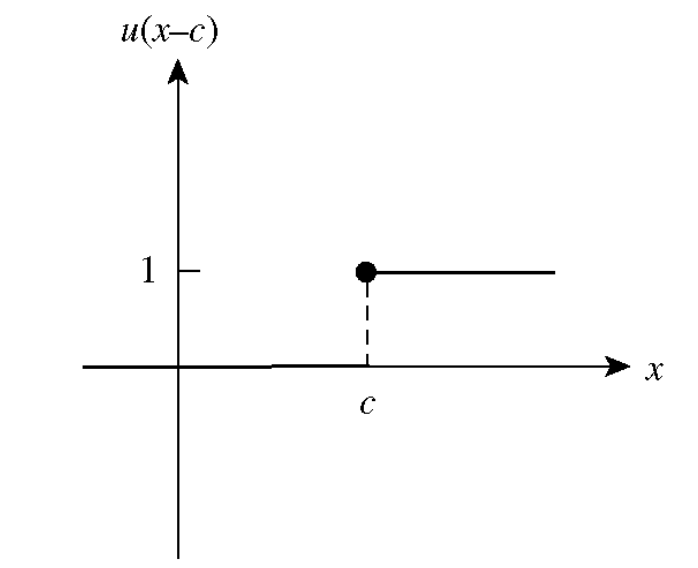
\includegraphics[height=5cm,keepaspectratio=true]{./edo/img0402.png}
		% img0402.png: 0x0 pixel, 300dpi, 0.00x0.00 cm, bb=
		\caption{Función Escalón $$u(x-c)$$}
		\label{fig:0402}
	\end{figure}
	



	\begin{thm}
		\label{bron:thm:23.3}
		$$
		\lap{u(x-c)}=\dfrac{1}{s}e^{-cs}.
		$$
	\end{thm}


\subsection{Traslaciones}


	Para cualquier funci\'on $f(x),$ definida para $x\geq0,$ obtenemos
	$$
	u(x-c)f(x-c)=
	\begin{cases}
	0 & x<c \\
	f(x-c) & x\geq c.
	\end{cases}
	$$



	\begin{figure}
		\centering
		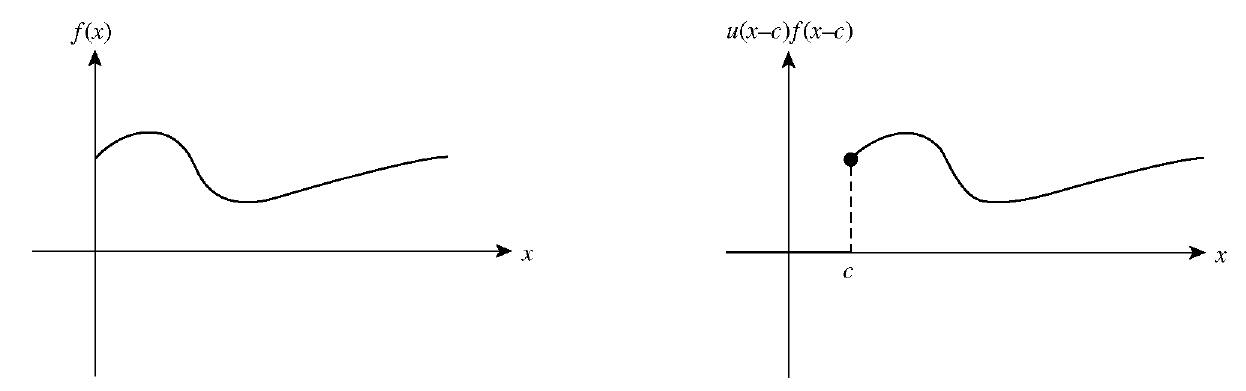
\includegraphics[height=3cm,keepaspectratio=true]{./edo/img0403.png}
		% img0403.png: 0x0 pixel, 300dpi, 0.00x0.00 cm, bb=
		\label{fig:0403}
	\end{figure}
	



	\begin{thm}
		\label{bron:thm:23.4}
		Si $F(s)=\lap{f(x)},$ entonces
		$$
		\lap{u(x-c)f(x-c)}=e^{-cs}F(s).
		$$
		
		De manera inversa
		$$\lapin{e^{-cs}F(s)}=u(x-c)f(x-c).$$
	\end{thm}
	


\subsection{Ejemplos}


	\begin{problema}
		\label{bron:exmp:23.1} Sean $f(x)=e^{3x}$ y $g(x)=e^{2x}.$
		\begin{enumerate}
			\item Calcule $f(x) \ast g(x);$
			\item calcule $g(x) \ast f(x);$
			\item verifique el teorema \ref{bron:thm:23.1}.
		\end{enumerate}
		
	\end{problema}
	



	\begin{problema}
		\label{bron:exmp:23.4}
		Encuentre
		$$
		\lapin{\dfrac{1}{s^{2}-5s+6}}
		$$
		\emph{por convoluciones.}
	\end{problema}
	



	\begin{problema}
		\label{bron:exmp:23.5}
		Encuentre
		$$
		\lapin{\dfrac{6}{s^{2}-1}}
		$$
		\emph{por convoluciones.}
	\end{problema}
	



	\begin{problema}
		\label{bron:exmp:23.6}
		Encuentre
		$$
		\lapin{\dfrac{1}{s\left( s^{2}+4 \right)}}
		$$
		\emph{por convoluciones.}
	\end{problema}
	



	\begin{problema}
		\label{bron:exmp:23.7}
		Encuentre
		$$
		\lapin{\dfrac{1}{\left( s-1 \right)^{2}}}
		$$
		\emph{por convoluciones.}
	\end{problema}
	



	\begin{problema}
		\label{bron:exmp:23.13}
		Encuentre $\lap{g(x)}$ si
		$$
		g(x)=\begin{cases}
		0 & x<4\\
		\left( x-4 \right)^{2} & x\geq 4.
		\end{cases}
		$$
	\end{problema}
	



	\begin{problema}
		\label{bron:exmp:23.14}
		Encuentre $\lap{g(x)}$ si
		$$
		g(x)=\begin{cases}
		0 & x<4\\
		x^{2} & x\geq 4.
		\end{cases}
		$$
	\end{problema}
	


%%%%%%%%%%%